\section{Computational lung models}
\label{section:review_models}
%
There exist a large number of computational ventilation and deformation models for the lung. Some models are designed to model particular phenomena whilst others are more general. They also range in spatial complexity from 0D compartment type models to 3D models which are able to incorporate `patient-specific' geometries extracted from CT images. In this review, we will focus on models that couple ventilation with tissue deformation and can be used as patient-specific models. %A review of popular compartment based lung models can be found in \citet{bates2009lung}. 
%
One study that couples ventilation and tissue deformation using a one way coupling approach is described in \citet{tawhai2010image}. Here a mechanics model for lung tissue is used to provide flow boundary conditions at terminal branches for an airway model. This makes the resultant ventilation distribution dependent on the tissue deformation, for example due to gravity. 
%
%In \citet{Swan2012}, air flow is simulated in patient specific conducting airways which are coupled to geometrically simplified terminal acinar units with varying volume dependent compliance. The fluid flow in the airways is approximated by Poiseuille flow with an added correction term for airway bifurcations. The end terminal acinar units are able to expand but are assumed to be independent of neighbouring acinar units. This does not allow for feedback from neighbouring acini that are in truth tightly connected by a matrix of fibers, collagen and capillaries. 
%
%This model confirms experimental evidence that in the healthy lungs tissue compliance has a far greater effect than airway resistance on the spatial distribution of ventilation, and hence a realistic description of tissue deformation is essential in models of ventilation. 
%
%
%Other sophisticated ventilation models of the whole airway tree, also exist \citep{yin2013multiscale,ismail2013coupled}. These models solve the full 3D Navier-Stokes equations in the upper airways, segmented from CT images, to capture high Reynolds number effects. The 3D fluid model is then coupled to a 0D laminar flow model of the lower airways.
%
Other sophisticated models of the whole lung that model ventilation and tissue deformation also exist \cite{ismail2013coupled,Swan2012}. Here the tissue is modelled by many independent elastic alveolar units. There is no clear way to conserve mass locally, so alveolar units can expand irrespectively of the size and position of neighbouring units. In reality the acini do not function as independent elastic balloons. They are physically coupled through fibrous scaffolding and shared alveolar septa. In our proposed model the tissue is modelled as one continuum, thus allowing us to conserve volume and couple neighbouring units. This is illustrated in Figure \ref{fig:balloons}. Also, these lung models \cite{ismail2013coupled,Swan2012} give information about the distribution of flow within the lung as a result of a pleural pressure boundary condition. However it is not possible to experimentally measure the pleural pressure in vivo using imaging or other apparatus. As part of the simulation protocol, the pleural pressure is therefore often tuned until physiological realistic flow rates are achieved. To overcome this issue, \cite{yin2013multiscale,yin2010simulation} proposed to estimate the flow boundary conditions for full organ ventilation models by means of image registration. However by solely relying on image registration to determine the ventilation distribution within the tissue one is not able to model the change in ventilation distribution due to progression of disease. In Chapter \ref{chap:lung} we will build on \cite{yin2010simulation} by integrating image registration based boundary conditions within the proposed poroelastic model of lung deformation. In particular, we propose to register expiratory images to the inspiratory images, to yield an estimate of the deformation boundary condition for the lung surface, and drive the simulation through this deformation boundary condition. Thus the tissue deformation and subsequent flow boundary condition for tree branches inside the lung and ventilation distribution is not pre-determined, but calculated from the coupled poroelastic-airway-tree model.

\begin{figure}[h]
\centering
   \subfloat[]{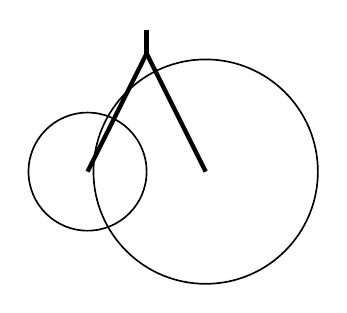
\begin{tikzpicture}[scale=1.5]
	\draw[ultra thick] (0.5,1) -- (0.5,1.2);
	\draw[ultra thick] (0.5,1) -- (0,0);
     	\draw[ultra thick] (0.5,1) -- (1,0);
\draw[semithick]  (0,0) circle [ultra thick,radius=0.5];
\draw[semithick]  (1,0) circle [ultra thick,radius=0.95];
\end{tikzpicture}
\label{fig:domains_cont}
}
  \subfloat[]{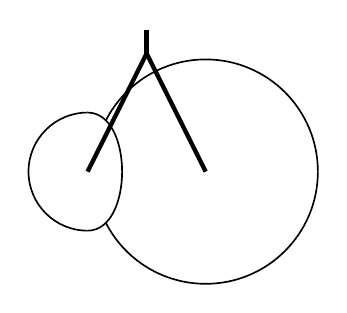
\begin{tikzpicture}[scale=1.5]
	\draw[ultra thick] (0.5,1) -- (0.5,1.2);
	\draw[ultra thick] (0.5,1) -- (0,0);
     	\draw[ultra thick] (0.5,1) -- (1,0);
\draw[semithick] (1.95,0) arc (0:153:0.95cm);
\draw[semithick] (1.95,0) arc (0:-153:0.95cm);
\draw[semithick] (0,0.5) arc (90:270:0.5cm);
%\draw (0,0.5) .. controls (0.5,0) and (0,-0.5) .. (0,-0.5);
\draw[semithick] (0,0.5) to [out=0,in=0] (0,-0.5) ; 
\end{tikzpicture}
\label{fig:domains_cont}
}
\caption{Sketch of two balloon models where the right unit is more compliant, thus being able to expand more easily. (a) Balloon model with independent alveolar units. The overlap in the alveolar units illustrates that mass is not conserved. (b) Balloon model where the alveolar units are coupled. Here the inflation of each alveolar unit is compromised by the expansion of its neighbor.}
\label{fig:balloons}
\end{figure}

 %None of these models incorporate the feedback of tissue deformation on ventilation and vice versa, and only loosely couple tissue deformation to ventilation.  


\section{Poroelastic models for lung parenchyma and other biological tissue}
%\label{section:poroelastic_review}
Some early work on a mechanical model of lung parenchyma as a poroelastic medium has already been proposed in \citet{kowalczyk1993mechanical}. This work developed a similar poroelastic model to the one we propose, however it has only been applied to a very simple 2D geometry. Also in \citet{owen2001mechanics} homogenisation theory has been used to derive macroscopic poroelastic equations for average air flows and tissue displacements in lung parenchyma during high frequency ventilation. The resulting model is a system of ordinary differential equations that is used to investigate the effect of high-frequency ventilation on strain in the parenchymal tissue. The use of a poroelastic model has also been applied to modelling other biological tissues. For example modelling protein based hydrogels embedded with cells \citep{galie2011linear}, perfusion of blood flow in the beating myocardium \citep{chapelle2010poroelastic,cookson2011novel}, the modelling of brain oedema (swelling) \citep{li2010three} and hydrocephalus \citep{wirth2006axisymmetric}. Another application is the modelling of interstitial fluid and tissue in articular cartilage and intervertebral discs \citep{mow1980biphasic,holmes1990nonlinear,galbusera2011comparison}.




\begin{comment}
%One study presented a framework for coupling models of ventilation and tissue deformation \cite{tawhai2006imaging}. First, changes in geometry of the lung mesh are determined and used to compute flow through an airway model. Pressures are then interpolated throughout the lung mesh to provide hydrostatic pressures that act as input loads for the mechanics model, which is then solved to predict shape change. These deformations are used to compute local volume changes which feed back as inputs to the flow-pressure problem and the system is solved iteratively. In these models tissue deformation is not directly dependent on ventilation, however an integrated model of ventilation and tissue mechanics model will be particularly important for understanding respiratory diseases since nearly all pulmonary diseases lead to some abnormality of lung tissue mechanics  \cite{suki2011lung}. For example, Chronic Obstructive Pulmonary Disease (COPD) encompasses emphysema (destruction of alveolar tissue) and chronic 
bronchitis which can cause severe bronchoconstriction and atelectasis (air trapping), both of which can significantly alter tissue properties. If the tissue mechanics are affected so too will the ventilation and vice versa emphasising the importance of a model that fully couples the tissue mechanics and ventilation in the lung. 

%There has been one study that presents a framework for coupling models of ventilation and tissue deformation \cite{tawhai2006imaging}. First, changes in geometry of the lung mesh are determined and used to compute flow through an airway model. Pressures are then interpolated throughout the lung mesh to provide hydrostatic pressures that act as input loads for the mechanics model, which is then solved to predict shape change. These deformations are used to compute local volume changes which feed back as inputs to the flow-pressure problem and the system is solved iteratively.

 %Although it is assumed that lung tissue is a continuum with uniform material properties, simulations of tissue deformation in a realistic geometry can give rise to a considerable degree of heterogeneity. 
%Including this model of tissue deformation in a ventilation model clearly predicts more physiologically consistent ventilation distributions than simply assuming that tissue compliance is constant or proportional to lung height. Therefore we conclude  that it is an essential feature in functional computational models of ventilation which aim to describe ventilation and perfusion matching or changes in ventilation distribution with disease.
%Another model that incorporates subject-specific anatomical geometry and approximates the airways by Poiseuille flow with an added correction term for airway bifurcations is presented in \cite{HedgesThesis}, here the aim is to predict forced expiration (FEV1) values. 

\end{comment}



 
%The model confirms experimental evidence that in the healthy lungs tissue
%compliance has a far greater effect than airway resistance on the spatial distribution of ventilation, and hence a realistic description of tissue deformation is essential in models of ventilation.
%Although it is assumed here that lung tissue is a continuum with uniform material properties, simulations of tissue deformation in a curvilinear geometry can give rise to a considerable degree of heterogeneity. Including this model of tissue deformation in a ventilation model clearly predicts more physiologically consistent ventilation distributions than simply assuming that tissue compliance is constant or proportional to lung height. Therefore we conclude  that it is an essential feature in functional computational models of ventilation which aim to describe ventilation and perfusion matching or changes in ventilation distribution with disease.''  \cite{SwanThesis}

 %However in this model, tissue deformation is not directly dependent on ventilation.


%Due to the often high Reynolds numbers in the upper airways, 3D fluid flow models have been used to model this sections of the airway tree. Clearly approximating the entire airway tree using 3D fluid flow remains intractable due to constraints on imaging resolution and computational power. Therefore smaller airways still need to be generated using a volume-filling branching algorithm \cite{tawhai2004ct} and then approximated by simpler 1D flow equations. The coupling of a 3D flow model to a 1D flow model for a complete airway tree has already been done in \cite{lin2009multiscale} and is achieved through mass conservation. i.e. the flow rates at the exit faces of the 3-D airway model can be determined by summing the flow rates at the terminal bronchioles using the connectivity information between the 3-D airway exit faces and the associated downstream 1-D airway branches. However this summing of flow rates is unable to account for any changes in resistances in the airway tree which might have been introduced 
%due to disease, for example bronchoconstriction or the collapsing of airways which is common in many types of COPD. There has also been sophisticated work on 3D to 1D fluid flow coupling for modelling blood flow with compliant vessels in the cardiovascular system \cite{formaggia2001coupling} and cerebral vasculature \cite{passerini20093d}.
